\documentclass[10pt,aspectratio=169]{beamer}
\usepackage{metrobridge}

\usepackage{chronology}
\usepackage{subcaption}

\usepackage{appendixnumberbeamer}
\usepackage{minted}
\setminted{escapeinside=||,linenos,breaklines,autogobble}

\usepackage[backend=biber, citestyle=authortitle, maxbibnames=99]{biblatex}
\renewcommand{\cite}{\footcite}
\renewcommand{\footnotesize}{\fontsize{6pt}{6pt}\selectfont}
\addbibresource{references.bib}

\title{Performance and Dynamism in User-extensible Compiler Infrastructures}
% \subtitle{An MPhil Thesis}
\date{June 19th 2025}
\author{Edmund Goodman} %, supervised by Dr Tobias Grosser and Sasha Lopoukhine}

\begin{document}

\maketitle
% \begin{frame}{Agenda}
%     \setbeamertemplate{section in toc}[sections numbered]
%     \tableofcontents
% \end{frame}


\begin{frame}{The modern compiler designer's challenge}
    % \begin{tikzpicture}[remember picture,overlay]
    %     \node[xshift=-1.1cm,yshift=-2.1cm] at (current page.north east) {
\includegraphics[width=0.125\textwidth]{images/sean_silva.jpg}};
    % \end{tikzpicture}
    \begin{figure}[H]
        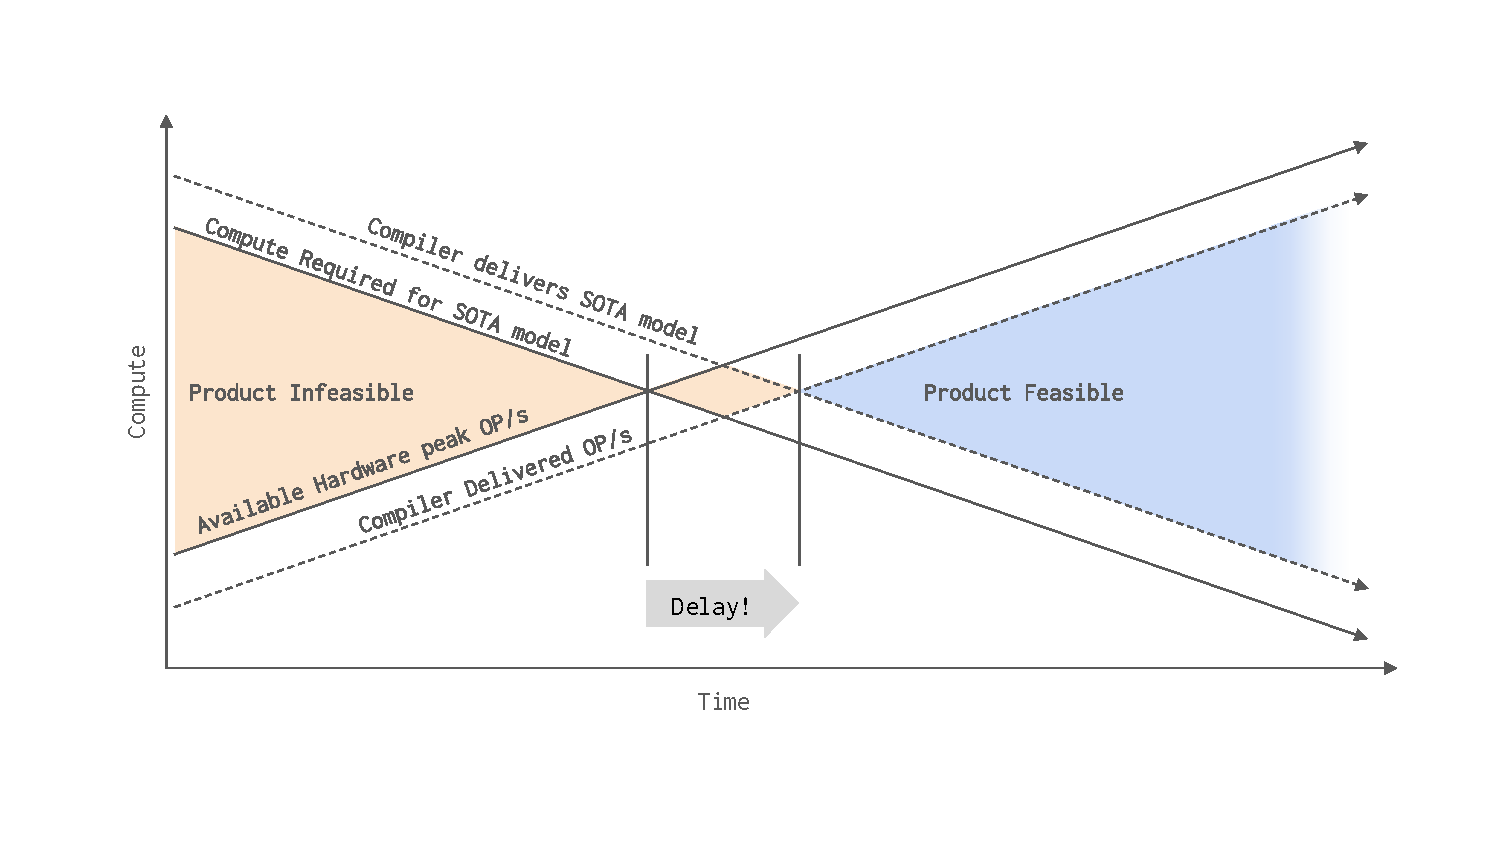
\includegraphics[width=0.8\textwidth]{images/compilers_lagging.pdf}
        \caption{Compilers are lagging behind the development of both machine
learning hardware and workloads. Figure created by Anton Lydike based on
a slide from a talk by Sean Silva’s talk\cite{seansilvaHighVelocityArchitectureMLIR2025}.}
        \label{fig:compilers_lagging}
    \end{figure}
\end{frame}

\begin{frame}[fragile]{An abridged history of compilers}
    \vspace{3em}
    \begin{chronology}*[5]{1950}{2025}{\textwidth}
        \event{1952}{A-0 System \cite{knuthEarlyDevelopmentProgramming1980}}%
        \event{1987}{GCC \cite{stallmanUsingGnuCompiler2009}}%
        % \event{1994}{SUIF \cite{wilsonSUIFInfrastructureResearch1994}}%
        \event{2002}{LLVM \cite{lattnerLLVMCompilationFramework2004}}%
        \event{2020}{MLIR \cite{lattnerMLIRScalingCompiler2021a}}%
        \event{2023}{xDSL \cite{fehrXDSLSidekickCompilation2025}}%
    \end{chronology}

    % \begin{enumerate}
    %     \item[1982] Early (spatial)
    % \end{enumerate}
    \vspace{1em}
\end{frame}


\begin{frame}[fragile]{MLIR \cite{lattnerMLIRScalingCompiler2021a}}
    \begin{columns}[T,onlytextwidth]
        \column{0.5\textwidth}
            % {\centering
\includegraphics[width=0.2\textwidth]{images/MLIR_Logo.png}}\\
            {\large \vspace{0.5em} \textbf{``A compiler infrastructure\\ for the 
            end of Moore's law''} \vspace{0.5em}}
            \vspace{1.25em}
            \begin{itemize}
                \itemindent=-13pt
                \item User-defined dialects
                \item Common shared infrastructure
                \item Highly optimised C++
                \begin{itemize}
                    \itemindent=-13pt
                    \item[$\Rightarrow$] Slow to build, but fast to run
                \end{itemize}
            \end{itemize}
        \column{0.5\textwidth}
            \begin{listing}[H]
                \centering
                \begin{minted}[fontsize=\scriptsize,xleftmargin=3em]{text}
                    builtin.module {
                      %0 = arith.constant 865 : i32
                      %1 = arith.constant 395 : i32
                      %2 = arith.addi %1, %0 : i32
                      %3 = arith.constant 777 : i32
                      %4 = arith.addi %3, %2 : i32
                      "test.op"(%4) : (i32) -> ()
                    }
                \end{minted}
                \caption{A program amenable to constant folding, expressed in MLIR's textual IR.}
                \label{listing:mlir-ir}
            \end{listing}
    \end{columns}
\end{frame}

\begin{frame}{xDSL \cite{fehrXDSLSidekickCompilation2025}}
    \begin{columns}[T,onlytextwidth]
        \column{0.5\textwidth}
            % {\centering
\includegraphics[width=0.2\textwidth]{images/xdsllogo.png}}\\
            \vspace{2em}
            {\large \textbf{A Python-native compiler framework, re-implementing MLIR’s data structures and logic}}
            \vspace{1.5em}
            \begin{itemize}
                \itemindent=-13pt
                \item Side-kick compiler for MLIR
                \item Runtime-extensible
                \item Readable Python%: fast to build and write, but slow to run?
                \begin{itemize}
                    \itemindent=-13pt
                    \item[$\Rightarrow$] Fast to build and write, but slow to run?
                \end{itemize}
            \end{itemize}
        \column{0.5\textwidth}
            \begin{figure}[H]
                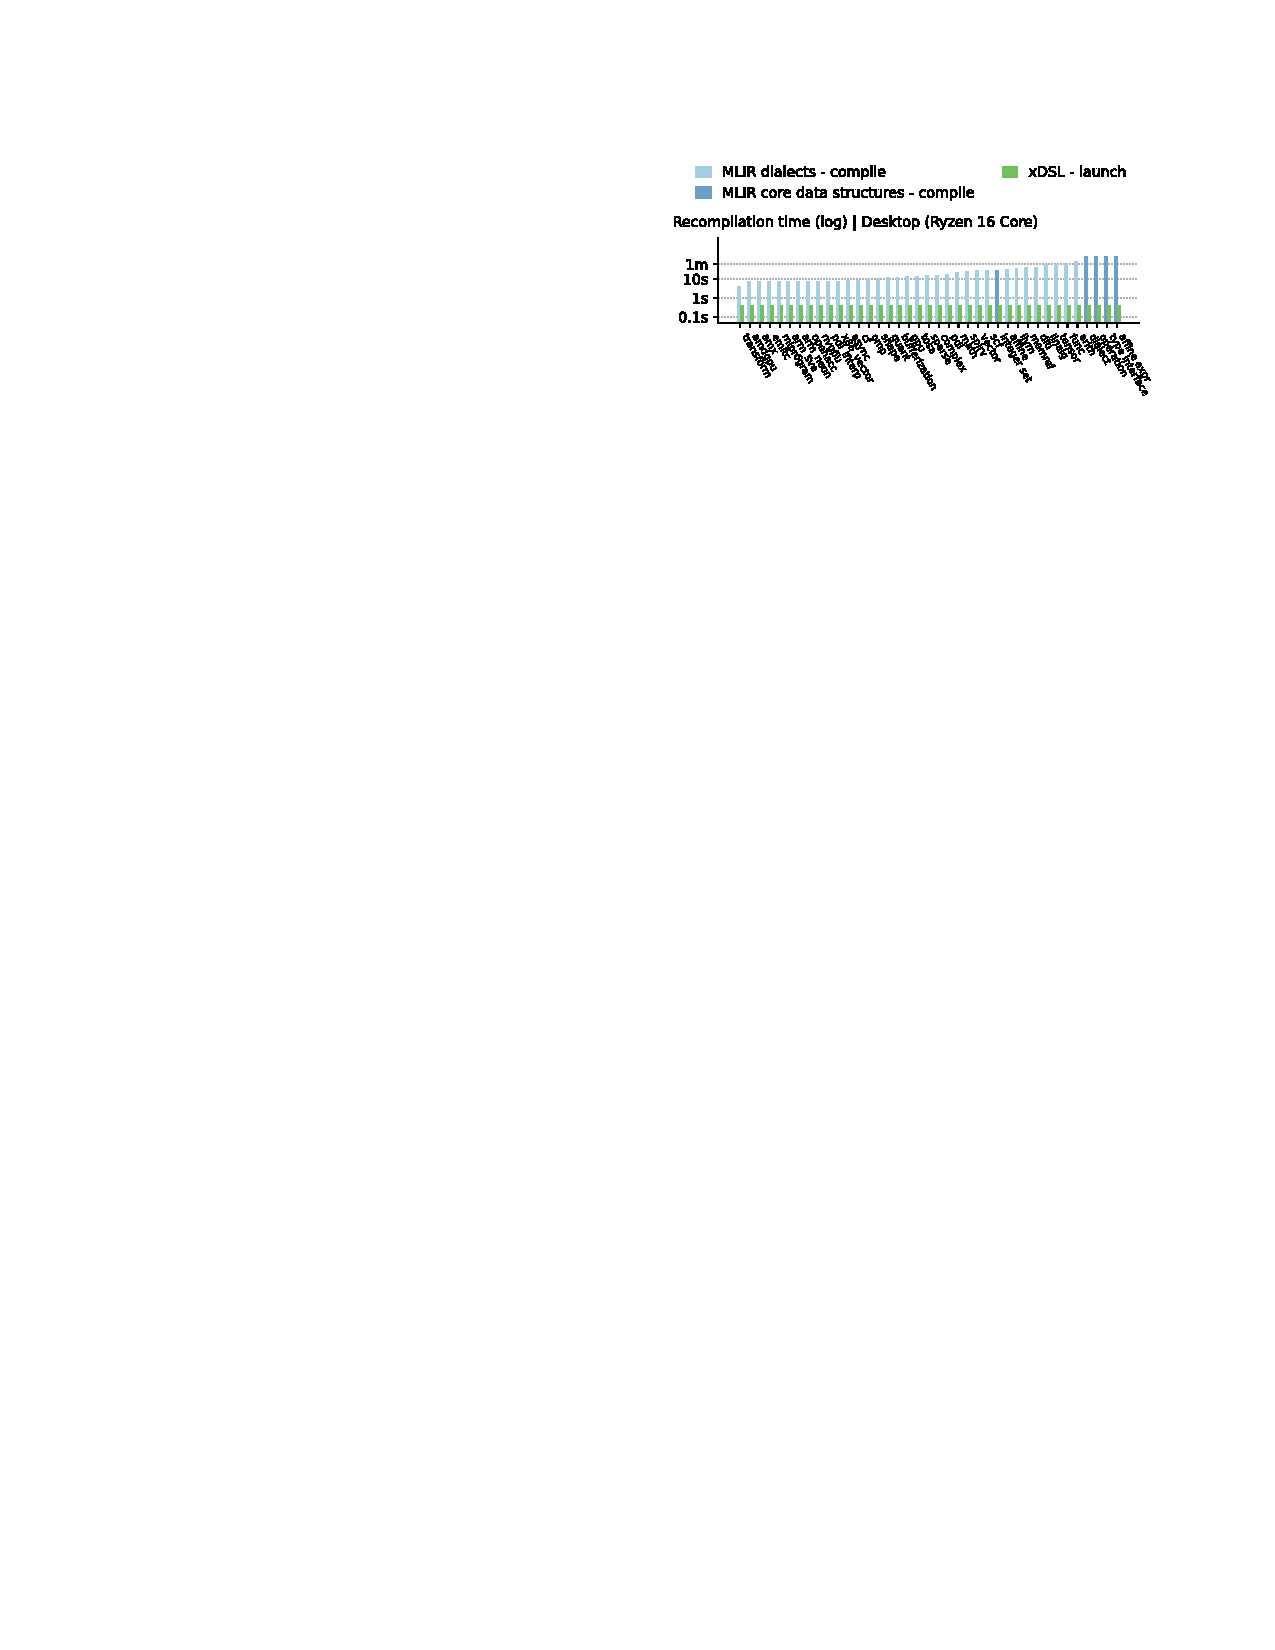
\includegraphics[width=\textwidth]{images/compile_times.pdf}
                \caption{``Recompiling MLIR after a single change is up
to two orders of magnitude slower than launching xDSL,
impacting prototyping and development efficiency'', Figure from xDSL paper \textsuperscript{8}.}
                \label{fig:compile_times}
            \end{figure}
        % \column{0.05\textwidth}
        % \column{0.45\textwidth}
    \end{columns}
\end{frame}


% \begin{frame}{xDSL \cite{fehrXDSLSidekickCompilation2025}}
%     \begin{figure}[H]
%         
\includegraphics[width=\textwidth]{images/compiling.png}
%         \caption{.}
%         \label{fig:compiling}
%     \end{figure}
% \end{frame}
% \begin{frame}{}
%     \begin{center}
%         \large A Python-native compiler framework, re-implementing MLIR’s data structures and logics
%     \end{center}
% \end{frame}

\begin{frame}{Key idea}
    \begin{center}
        \huge Pointer-chasing, unstructured workloads are hard to optimise ahead-of-time
    \end{center}
    \vspace{1em}

    \begin{itemize}
        \item Pointer-chasing workloads are bottlenecked by memory accesses\cite{wangEvaluatingSynchronizationOverhead2025}
        \item Runtime control flow incurs overhead and precludes optimisations \cite{driesenDirectCostVirtual1996}  \cite{emerybergerPythonPerformanceMatters2022}
        % \vspace{0.5em}
        \item \textit{MLIR and xDSL are both examples of this workload type}
    \end{itemize}
\end{frame}

\begin{frame}{Research question}
    \begin{center}
        \huge How much does writing your compiler in a dynamic language actually slow it down? \\
    \end{center}
    \vspace{1.5em}

    \begin{itemize}
        % \item Is this slow-down justified by easy runtime extensibility and fast development cycles?
        \item Let's measure this, using MLIR and xDSL as proxies for static and dynamic languages
        \item Is this slow-down matched by other benefits of dynamic languages?
    \end{itemize}
\end{frame}


% \begin{frame}{Contributions}
%     \begin{columns}[T,onlytextwidth]
%         \column{0.5\textwidth}
%             \vspace{3em}
%             \begin{enumerate}
%                 % \item An examination of the current %and best-case performance of pattern rewriting workloads in the CPython language runtime.
%                 \item Measured current and best-case performance of MLIR and xDSL
%                 % \item A tool to examine CPython bytecode dispatch in program runs, facilitating the analysis of costs incurred by dynamism.
%                 \item Built tool to examine Python at the bytecode level
%                 % \item A specialisation of the current xDSL implementation for pattern rewriting workloads, demonstrating the best-case performance of CPython for such applications.
%                 \item Examined impact of dynamic optimisations on xDSL
%                 % \item An exploration of optimisation techniques to shrink the performance gap between dynamic and static languages for pattern rewriting workloads.
%                 \item Investigated cost of dynamism for compiler frameworks
%                 % \item A quantitative comparison of the performance of user-extensible compiler frameworks implemented in static and dynamic languages, focussing on the impact of dynamism. % leveraging sidekick compilation for fine-grained analysis of the impact of dynamisms
%             \end{enumerate}
%         \column{0.5\textwidth}
%             \begin{figure}[H]
%                 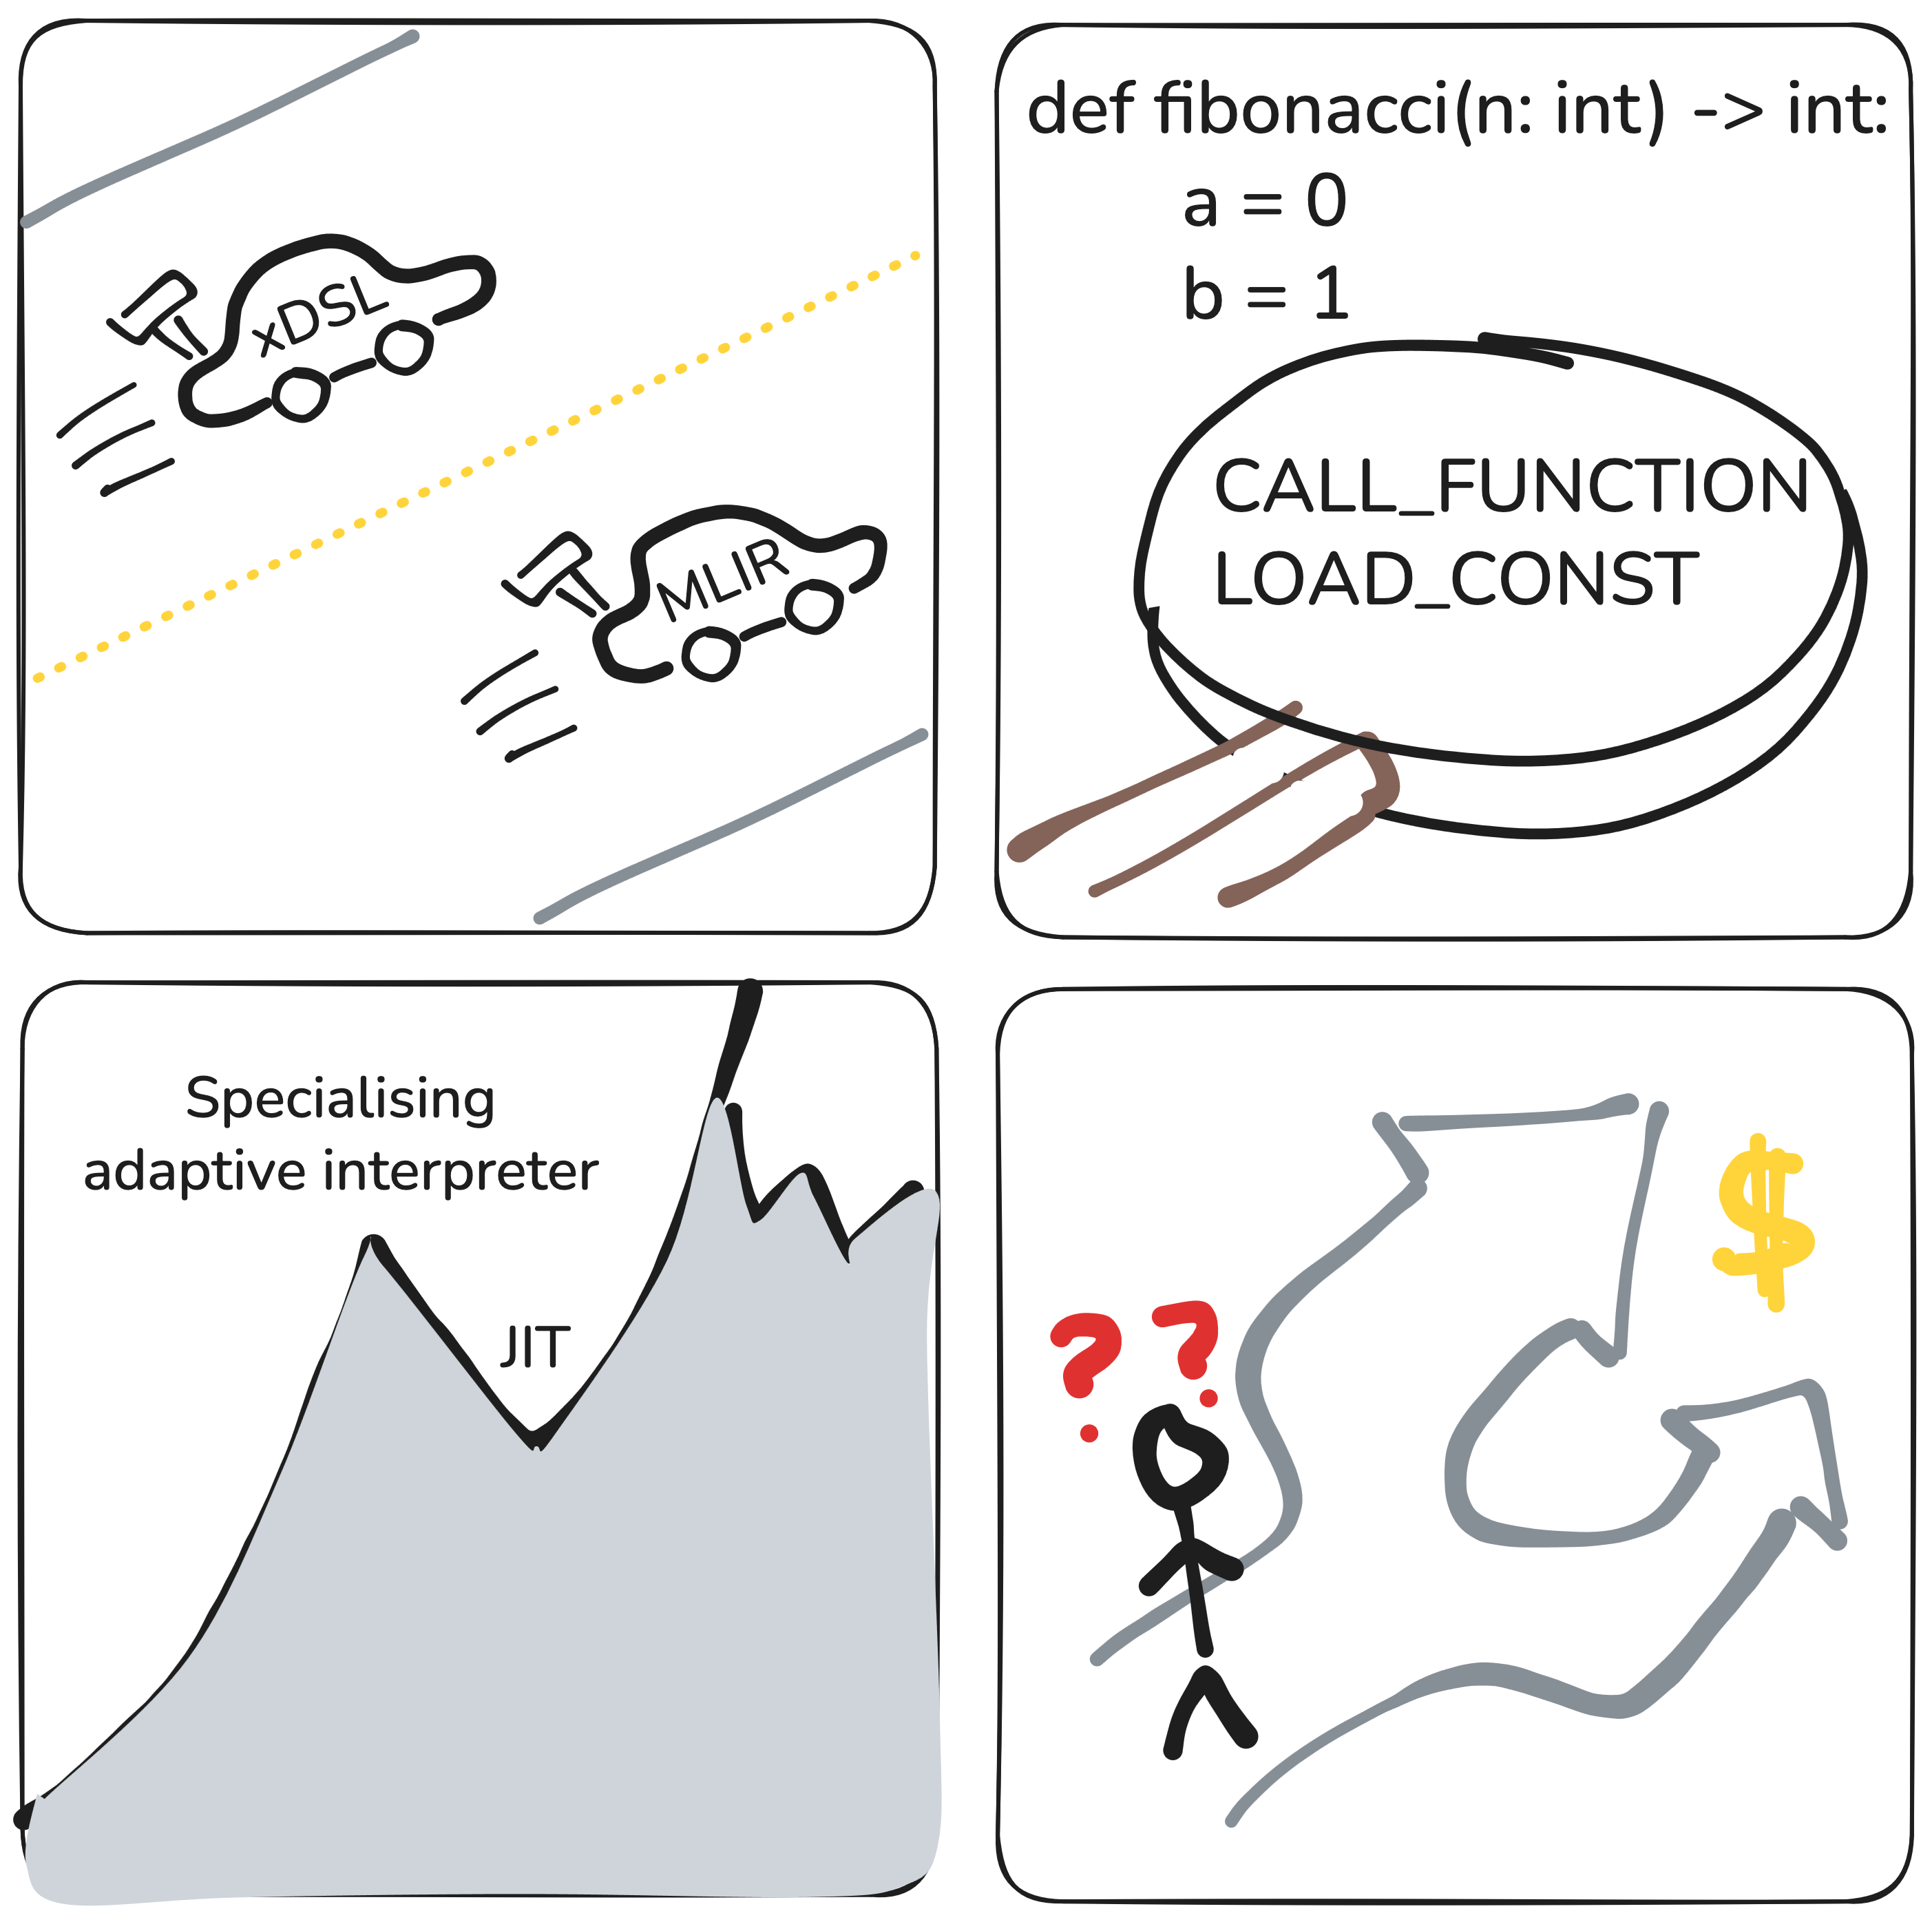
\includegraphics[width=0.8\textwidth]{images/contributions.png}
%                 \label{fig:contributions}
%             \end{figure}
%     \end{columns}
% \end{frame}

\begin{frame}{Contributions}
    \Large
    \begin{enumerate}
        \item Comparison of MLIR and xDSL performance
        \vspace{0.5em}
        \item Tool to examine Python at the bytecode level
        \vspace{0.5em}
        \item Impact of dynamic optimisations on xDSL
        \vspace{0.5em}
        \item Cost of dynamism for compiler frameworks
        % \item Compared performance of MLIR and xDSL
        % \vspace{0.5em}
        % \item Built tool to examine Python at the bytecode level
        % \vspace{0.5em}
        % \item Examined impact of dynamic optimisations on xDSL
        % \vspace{0.5em}
        % \item Investigated cost of dynamism for compiler frameworks
    \end{enumerate}
\end{frame}



\begin{frame}{Performance of MLIR and xDSL}
    \begin{columns}[T,onlytextwidth]
        \column{0.5\textwidth}
            \begin{itemize}
                \vspace{2em}
                \itemindent=-13pt
                \item Measure with micro-benchmarks \cite{aminiHowSlowMLIR2024}, and end-to-end optimisation workloads
                \vspace{1.5em}
                \item Current xDSL $100\times$ slower than MLIR
                \begin{itemize}
                    \itemindent=-13pt
                    \item Also measures implementation details
                \end{itemize}
                \item Specialised xDSL $14\times$ slower than MLIR
                \begin{itemize}
                    \itemindent=-13pt
                    \item Proxy for static and dynamic languages
                \end{itemize}
                \item Contrast $60,000\times$ slower for GEMM \cite{emerybergerPythonPerformanceMatters2022}
            \end{itemize}
            \vspace{1em}
        \column{0.5\textwidth}
            \vspace{1em}
            \begin{figure}[H]
                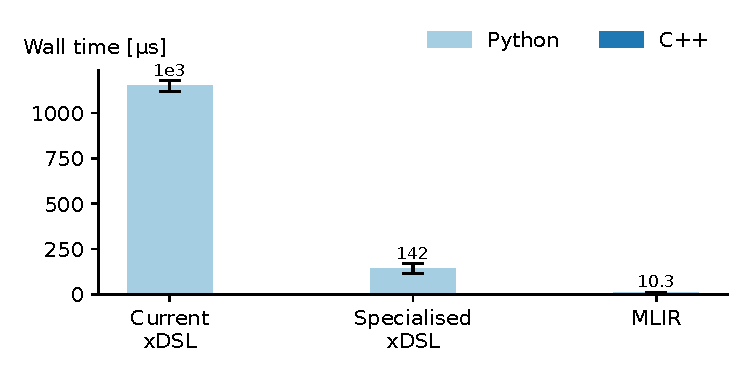
\includegraphics[width=\textwidth]{images/constant_performance.pdf}
                \caption{Performance of constant folding over twenty integer additions.}
                % \caption{Constant folding over integer addition in xDSL is $100\times$ slower than MLIR, but specialisation can improve this to only $14\times$ slower.}
                % \caption{Specialisation of constant folding over integer addition in xDSL yields performance uplifts of up to $8\times$, $14\times$ slower than the MLIR reference implementation.}
                \label{fig:constant_performance}
            \end{figure}
    \end{columns}
\end{frame}

\begin{frame}[fragile]{Examining Python bytecode}
    \begin{figure}[H]
        \centering
        \begin{subfigure}[b]{0.275\textwidth}
           \centering
            \begin{minted}[fontsize=\scriptsize]{python}
    import bytesight
    
    def inner_function(x):
        assert x
    
    def example_function():
        inner_function(1)
    
    bytesight.profile_bytecode(
        example_function
    )
            \end{minted}
            \footnotesize\vspace{2em}
            \caption{Python program.}
            \label{listing:profiler-example-python}
        \end{subfigure}
        \hfill
        \begin{subfigure}[b]{0.7\textwidth}
            \centering
            \begin{minted}[fontsize=\scriptsize,linenos=false]{text}
    // ======= example:6 `example_function` ========
    // >>> inner_function(1)
    7           0   LOAD_GLOBAL          0   (inner_function) // 15 ns
                2   LOAD_CONST           1   (1)              // 15 ns
                4   CALL_FUNCTION        1   ()               // 31 ns
        // ======== example:3 `inner_function` =========
        // >>> assert x
        4           0   LOAD_FAST            0   (x)          // 13 ns
                    2   POP_JUMP_IF_TRUE     4   (to 8)       // 13 ns
                >>  8   LOAD_CONST           0   (None)       // 12 ns
                    10  RETURN_VALUE             ()           // 31 ns
        // =============================================
                6   POP_TOP                  ()               // 16 ns
                18  RETURN_VALUE             ()               // 28 ns
    // =============================================
            \end{minted}
            \caption{Profiler output.}
            \label{listing:profiler-example-bytecode}
        \end{subfigure}
        \vspace{-0.5em}
        \captionsetup{name=Listing}
        \caption{Our novel performance profiler, ByteSight, shows the sequence of dispatched bytecode and their individual execution times for Python programs.}
        \label{listing:profiler-example}
    \end{figure}
\end{frame}

\begin{frame}{Impact of dynamic optimisations on xDSL}
    \begin{columns}[T,onlytextwidth]
        \column{0.475\textwidth}
            \begin{itemize}
                \itemindent=-13pt
                \item Assess impact of CPython optimisations leveraging runtime information
                % \item Faster CPython implements optimisations leveraging runtime information
                % \item JIT causes regressions as WIP infrastructure
                \item Use PyPerformance \cite{collinwinterPythonPyperformance2025} benchmarks as a baseline for average workloads
                % \item PyPerformance \cite{collinwinterPythonPyperformance2025} provides a suite of real-world benchmarks
                \vspace{1em}
                \item xDSL yields $\sim5\%$ greater change than the average workload
                \item Specialised xDSL even more amenable to optimisation, up to $\sim11\%$ speedup
            \end{itemize}
        \column{0.025\textwidth}
        \column{0.5\textwidth}
            \begin{figure}[H]
                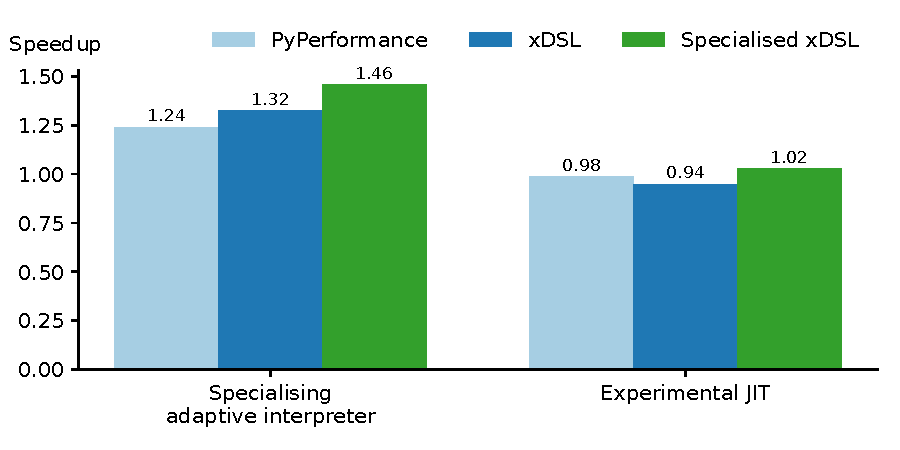
\includegraphics[width=\textwidth]{images/15_summary.pdf}
                \caption{Speed-up from optimisations across workloads.}
                % \caption{Dynamic workloads like constant folding in xDSL exacerbate the performance impact of CPython optimisations leveraging runtime information, with manual specialisation further revealing optimisation opportunities.}
                \label{fig:15_summary}
            \end{figure}
    \end{columns}
\end{frame}

\begin{frame}{Cost of dynamism in compiler frameworks}
    \begin{columns}[T,onlytextwidth]
        \column{0.5\textwidth}
            \vspace{2em}
            \begin{figure}[H]
                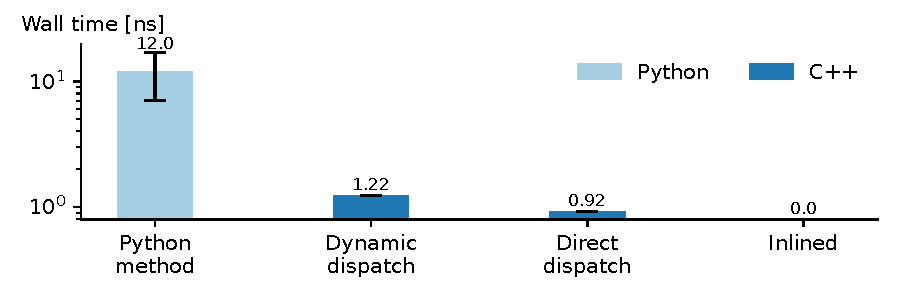
\includegraphics[width=\textwidth]{images/dispatch.pdf}
                \caption{Measuring dynamic function dispatch performance for Python 3.10 and \texttt{clang -O3}.}
                % \caption{Dynamic dispatch generated by \texttt{clang -O3} incurs a $30\%$ overhead in comparison with direct dispatch, but remains an order of magnitude more performant than CPython 3.10 method invocation.}
                \label{fig:dispatch}
            \end{figure}
        \column{0.5\textwidth}
            \begin{itemize}
                \item Can quantify exact costs of specific dynamic components, for example
                \vspace{1em}
                \item C++ dynamic dispatch incurs overhead due to:
                \begin{enumerate}
                    \item Indirection through the vTable\cite{driesenDirectCostVirtual1996}
                    \item Precluding optimisations like function inlining
                \end{enumerate}
                \item Python dynamically dispatches all functions, incurring a high overhead
            \end{itemize}
    \end{columns}
\end{frame}


\begin{frame}{Conclusions}
    \begin{columns}[T,onlytextwidth]
        \column{0.5\textwidth}
            \vspace{3em}
            \begin{itemize}
% Our work identifies dynamism in user-extensible compiler infrastructures as a result of the
% heterogeneous data structures used to represent IR, whose structure and contents is known
% only at runtime. It then quantifies the performance cost this dynamism incurs in their
% ahead-of-time compiled implementation. We contrast this with implementations in dynamic
% languages, empirically demonstrating that the performance overhead typically associated
% with such languages is lessened by both the workload’s dynamic nature, and modern
% optimisation approaches to dynamic language runtimes. This contribution challenges the
% status quo of implementing user-extensible compiler frameworks in static, ahead-of-time
% compiled languages, typified by LLVM’s MLIR in C++. Instead, we motivate the use of
% dynamic languages for these frameworks, showing that implementations such as xDSL
% which follow this approach present a desirable balance of framework performance with the
% developer productivity required to deliver modern workloads without delay.

                % \item Dynamic languages can approach static performance, as compilers are hard to ahead-of-time optimise
                % \item Dynamic languages balance performance with productivity
                \itemindent=-13pt
                \item Compiler frameworks get less benefit out of ahead-of-time optimisations than more static workloads
                \item Dynamic languages provide other benefits, aiding development velocity
                \vspace{1.5em}
                \item \textit{Challenge the status quo of writing compiler frameworks in static languages}
            \end{itemize}
        \column{0.5\textwidth}
            \begin{figure}[H]
                \vspace{-1em}
                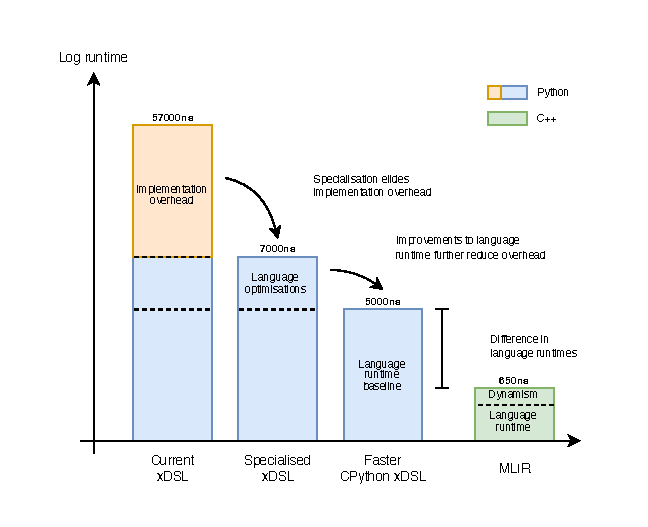
\includegraphics[width=\textwidth]{images/narrative.drawio.pdf}
                \vspace{-1.5em}
                \caption{Closing the gap between xDSL and MLIR pattern rewriting performance.} % xDSL’s performance can be improved by changes to both its implementation and language runtime. C++ has less of a performance advantage for MLIR than other workloads due to the costs associated with dynamism.}
                \label{fig:narrative}
            \end{figure}
    \end{columns}
    % Summary sentence
    % \begin{itemize}
    %     \item[$\Rightarrow$] Result
    % \end{itemize}
\end{frame}

\begin{frame}{Impact and future work}
    \begin{figure}[H]
        % \hspace*{-1.75cm}
        % 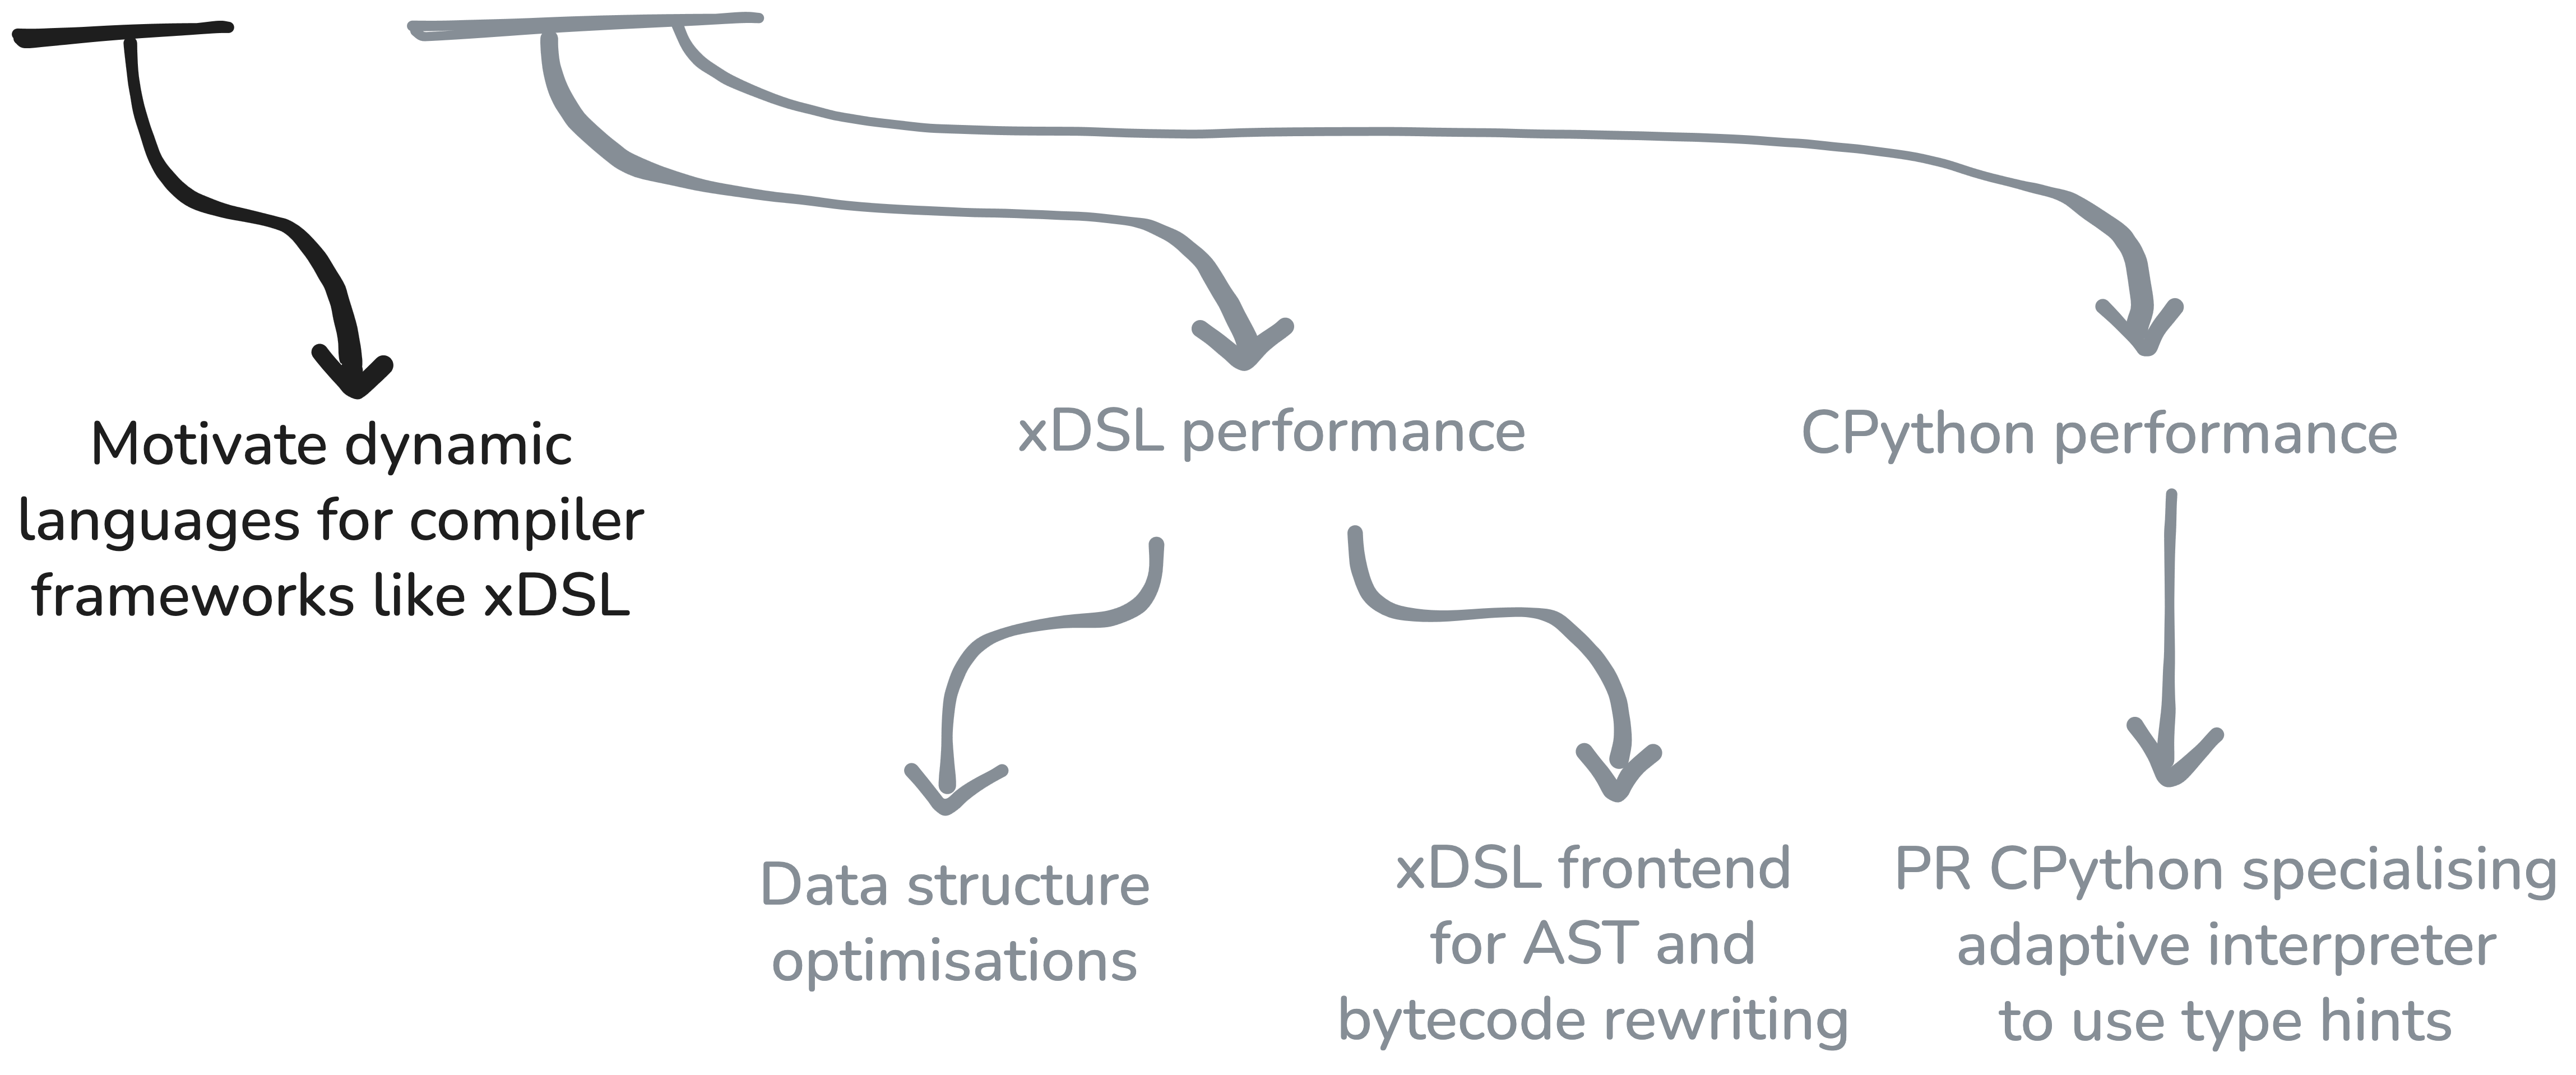
\includegraphics[width=\textwidth]{images/impact_future_work.png}
        % \vspace{2cm}
        \hspace*{-1cm}
        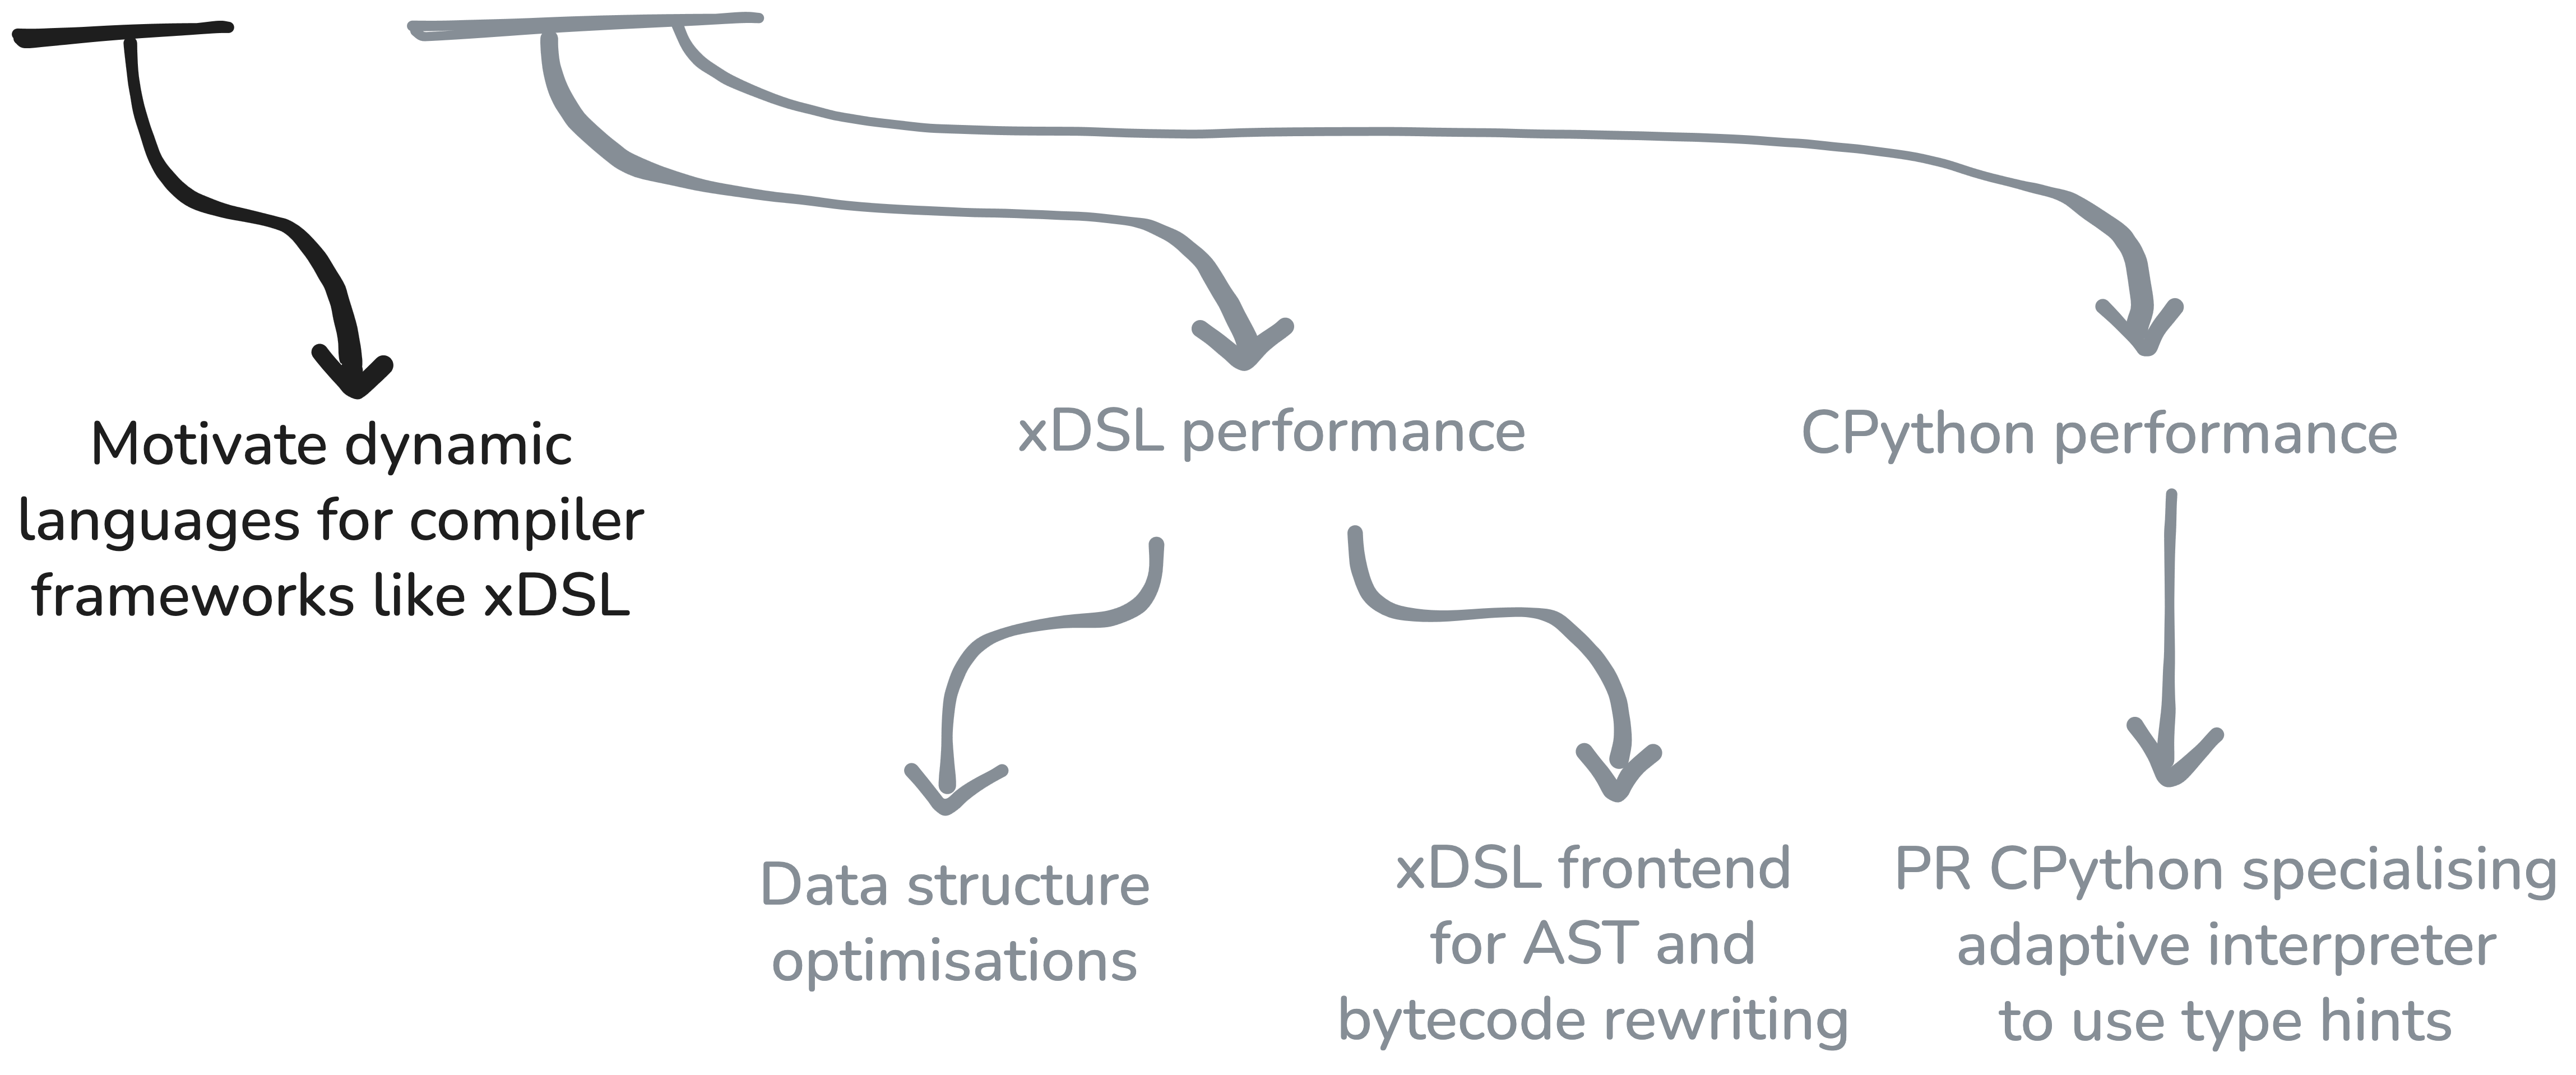
\includegraphics[width=\textwidth]{images/impact_future_work.png}
        \vspace{2cm}
    \end{figure}
\end{frame}


\appendix

\maketitle

\begin{frame}[allowframebreaks]{References}
    \printbibliography[heading=none]
\end{frame}

\end{document}


% =============================================================== %
% More example slides, derived from https://www.overleaf.com/latex/templates/metropolis-beamer-theme/qzyvdhrntfmr %
% =============================================================== %

% \begin{frame}{Bullets}
%     \begin{itemize}
%         \item This is a bullet \alert{point}
%         \item This is another bullet point
%     \end{itemize}
% \end{frame}

% \begin{frame}{Columns}
%     \begin{columns}[T,onlytextwidth]
%         \column{0.5\textwidth}
%             \textbf{Items}
%             \begin{itemize}
%                 \item Milk
%                 \item Eggs
%                 \item Potatoes
%             \end{itemize}
        
%         \column{0.5\textwidth}
%             \textbf{Enumerations}
%             \begin{enumerate}
%                 \item First,
%                 \item Second,
%                 \item and Last.
%             \end{enumerate}
%     \end{columns}
% \end{frame}

% \begin{frame}{Images}
%     \begin{figure}[H]
%         \includegraphics[width=0.45\textwidth]{example-image-a}
%         \caption{A caption \cite{Knuth92}.}
%         \label{fig:image}
%     \end{figure}
% \end{frame}

% \begin{frame}[fragile]{Code}
%     \begin{listing}[H]
%         \begin{minted}[linenos=false]{haskell}
%             newtype Lasagne = Lasagne Int
%                 deriving (Show, Num)
            
%             -- The stacking operating can be considered integer 
%             -- addition of the number of layers
%             instance Semigroup Lasagne where
%                 (<>) = (+)
%         \end{minted}
%         \caption{Another caption.}
%         \label{lst:listing}
%     \end{listing}
% \end{frame}

% =============================================================== %

% \begin{frame}{Blocks}
%   Three different block environments are pre-defined and may be styled with an optional background color.
%   \metroset{block=fill}
%   \begin{block}{Default}
%     Block content.
%   \end{block}
%   \begin{alertblock}{Alert}
%     Block content.
%   \end{alertblock}
%   \begin{exampleblock}{Example}
%     Block content.
%   \end{exampleblock}
% \end{frame}

% \begin{frame}[fragile]{Typography}
%       \begin{verbatim}The theme provides sensible defaults to
% \emph{emphasize} text, \alert{accent} parts
% or show \textbf{bold} results.\end{verbatim}

%   \begin{center}becomes\end{center}

%   The theme provides sensible defaults to \emph{emphasize} text,
%   \alert{accent} parts or show \textbf{bold} results.
% \end{frame}

% \begin{frame}{Animation}
%   \begin{itemize}[<+- | alert@+>]
%     \item \alert<4>{This is\only<4>{ really} important}
%     \item Now this
%     \item And now this
%   \end{itemize}
% \end{frame}

% \begin{frame}{Font feature test}
%   \begin{itemize}
%     \item Regular
%     \item \textit{Italic}
%     \item \textsc{SmallCaps}
%     \item \textbf{Bold}
%     \item \textbf{\textit{Bold Italic}}
%     \item \textbf{\textsc{Bold SmallCaps}}
%     \item \texttt{Monospace}
%     \item \texttt{\textit{Monospace Italic}}
%     \item \texttt{\textbf{Monospace Bold}}
%     \item \texttt{\textbf{\textit{Monospace Bold Italic}}}
%   \end{itemize}
% \end{frame}

% \begin{frame}{Figures}
%   \begin{figure}
%     \newcounter{density}
%     \setcounter{density}{20}
%     \begin{tikzpicture}
%       \def\couleur{alerted text.fg}
%       \path[coordinate] (0,0)  coordinate(A)
%                   ++( 90:5cm) coordinate(B)
%                   ++(0:5cm) coordinate(C)
%                   ++(-90:5cm) coordinate(D);
%       \draw[fill=\couleur!\thedensity] (A) -- (B) -- (C) --(D) -- cycle;
%       \foreach \x in {1,...,40}{%
%           \pgfmathsetcounter{density}{\thedensity+20}
%           \setcounter{density}{\thedensity}
%           \path[coordinate] coordinate(X) at (A){};
%           \path[coordinate] (A) -- (B) coordinate[pos=.10](A)
%                               -- (C) coordinate[pos=.10](B)
%                               -- (D) coordinate[pos=.10](C)
%                               -- (X) coordinate[pos=.10](D);
%           \draw[fill=\couleur!\thedensity] (A)--(B)--(C)-- (D) -- cycle;
%       }
%     \end{tikzpicture}
%     \caption{Rotated square from
%     \href{http://www.texample.net/tikz/examples/rotated-polygons/}{texample.net}.}
%   \end{figure}
% \end{frame}
% \begin{frame}{Tables}
%   \begin{table}
%     \caption{Largest cities in the world (source: Wikipedia)}
%     \begin{tabular}{lr}
%       \toprule
%       City & Population\\
%       \midrule
%       Mexico City & 20,116,842\\
%       Shanghai & 19,210,000\\
%       Peking & 15,796,450\\
%       Istanbul & 14,160,467\\
%       \bottomrule
%     \end{tabular}
%   \end{table}
% \end{frame}

% \begin{frame}{Math}
%   \begin{equation*}
%     e = \lim_{n\to \infty} \left(1 + \frac{1}{n}\right)^n
%   \end{equation*}
% \end{frame}

% \begin{frame}{Line plots}
%   \begin{figure}
%     \begin{tikzpicture}
%       \begin{axis}[
%         mlineplot,
%         width=0.9\textwidth,
%         height=6cm,
%       ]

%         \addplot {sin(deg(x))};
%         \addplot+[samples=100] {sin(deg(2*x))};

%       \end{axis}
%     \end{tikzpicture}
%   \end{figure}
% \end{frame}

% \begin{frame}{Bar charts}
%   \begin{figure}
%     \begin{tikzpicture}
%       \begin{axis}[
%         mbarplot,
%         xlabel={Foo},
%         ylabel={Bar},
%         width=0.9\textwidth,
%         height=6cm,
%       ]

%       \addplot plot coordinates {(1, 20) (2, 25) (3, 22.4) (4, 12.4)};
%       \addplot plot coordinates {(1, 18) (2, 24) (3, 23.5) (4, 13.2)};
%       \addplot plot coordinates {(1, 10) (2, 19) (3, 25) (4, 15.2)};

%       \legend{lorem, ipsum, dolor}

%       \end{axis}
%     \end{tikzpicture}
%   \end{figure}
% \end{frame}

% {%
% \setbeamertemplate{frame footer}{My custom footer}
% \begin{frame}[fragile]{Frame footer}
%     Metropolis defines a custom beamer template to add a text to the footer. It can be set via
%     \begin{verbatim}\setbeamertemplate{frame footer}{My custom footer}\end{verbatim}
% \end{frame}
% }

% \begin{frame}{References}
%   Some references to showcase [allowframebreaks] \cite{knuth92,ConcreteMath,Simpson,Er01,greenwade93}
% \end{frame}

% \begin{frame}[fragile]{Backup slides}
%   Sometimes, it is useful to add slides at the end of your presentation to
%   refer to during audience questions.

%   The best way to do this is to include the \verb|appendixnumberbeamer|
%   package in your preamble and call \verb|\appendix| before your backup slides.

%   Metropolis will automatically turn off slide numbering and progress bars for
%   slides in the appendix.
% \end{frame}
